\section{Литералы в Haskell}

\subsection{Классификация}

В Хаскель можно выделить четыре вида литералов: целочисленные, вещественные,
символьные и строковые.

В отличие от многих других языков, логические значения \texttt{True} и
\texttt{False} являются идентификаторами. Они входят в состав стандартного
модуля \texttt{Prelude} и определены как показано в листинге \ref{lst:bool}.

\begin{ListingEnv}
\begin{lstlisting}[language=Haskell]
data Bool = True | False
\end{lstlisting}
\caption{Определение значений True и False}
\label{lst:bool}
\end{ListingEnv}

Целочисленные литералы представляют значения натуральных чисел, включая ноль.
Существует синтаксис для записи в различных системах счисления: десятичной,
восьмеричной, шестнадцатеричной. Примеры: \texttt{15}, \texttt{0o17},
\texttt{0O17}, \texttt{0xF}, \texttt{0XF}.

\begin{figure}[H]
\centering
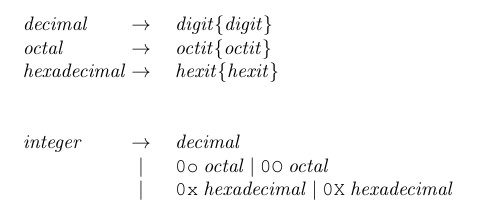
\includegraphics[scale=0.7]{pic-integral-literals}
\caption{Лексическая структура целочисленных литералов\cite{haskell2010}}
\end{figure}

Вещественные литералы представляют рациональные числа. Можно использовать как
обычные десятичные дроби, так и научную форму записи с указанием мантиссы и
порядка. Примеры: \texttt{123.456}, \texttt{0.123456e3}.

\begin{figure}[H]
\centering
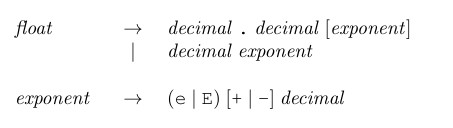
\includegraphics[scale=0.7]{pic-rational-literals}
\caption{Лексическая структура вещественных литералов\cite{haskell2010}}
\end{figure}

Символьные литералы записываются в одинарных кавычках, а строковые в двойных.
Примеры: \texttt{'a'}, \texttt{"Hello, World!"}.

\begin{figure}[H]
\centering
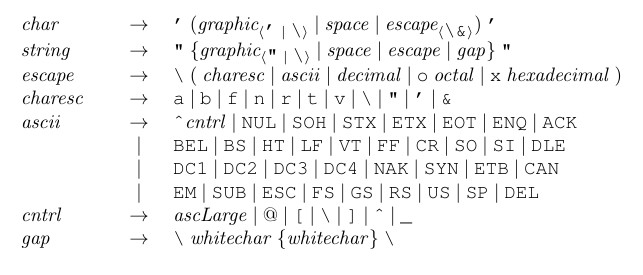
\includegraphics[scale=0.7]{pic-char-string-literals}
\caption
{Лексическая структура символьных и строковых литералов\cite{haskell2010}}
\end{figure}

\subsection{Отрицательные числа}

Как можно заметить из приведённых фрагментов стандарта, знак не является частью
лексемы обозначающей число. Тем не менее запиь \texttt{-10} является
синтаксически правильной. Минус в данном случае является отдельной лексемой,
обозначающей операцию унарный минус. Во время компиляции он заменяестя вызовом
функции \texttt{negate}, определённой в классе \texttt{Num} стандартного модуля
\texttt{Prelude}.

Вместе с другими особенностями синтаксиса и системы типов это рождает некоторые
трудности.

\subsection{Особенность 1: вызов функции записывается без скобок}

Функции играют в языке Хаскель важную роль. Для такого частого действия, как
вызов функции, разработчики решили сделать максимально простой синтаксис.
Чтобы вызвать фукнцию \texttt{f} с аргументом \texttt{x}, достаточно просто
написть \texttt{f x}.

Листинг \ref{lst:space} демонстрирует пробему, связанную с отсутствием
необходимости писать скобки вокруг аргументов. Выражение \texttt{print -1}
вопринимается компилятором, как вызов функции \texttt{print} с двумя
аргументами: \texttt{-} и \texttt{1}. Такое действие невозможно, о чём нам
любезно сообщает компилятор. Вероятно, программист хотел напечатать число минус
один. Для того чтобы сделать это, ему необоходимо обернуть \texttt{-1} в
скобки, то есть написать \texttt{print (-1)}.

\begin{ListingEnv}[H]
\begin{lstlisting}
Prelude> print (-1) -- OK
Prelude> print -1   -- ERROR
\end{lstlisting}
\begin{verbatim}
<interactive>:2:1:
    Non type-variable argument in the constraint:
                                Num (a -> IO ())
    (Use FlexibleContexts to permit this)
    When checking that ‘it’ has the inferred type
      it :: forall a. (Num (a -> IO ()), Show a)
            => a -> IO ()
\end{verbatim}
\caption{Ошибка при отсутствии скобок вокруг унарного минуса}
\label{lst:space}
\end{ListingEnv}

Стоит сказать, что многие программисты на Хаскель стараются не писать лишних
скобок. Для них необходимость оборачивать отрицательные числа в скобки может
может быть раздражающей и даже мешающей, ухудшающей читаемость кода.

\subsection{Особенность 2: тип значения представляемого литералом определяется
контекстом}

Система типов языка Хаскель позволяет литералам иметь разный тип в разных
контекстах. Сами по себе целочисленные и вещественные литералы не имеют
конкретного предопределённого типа. Он определяется во время компиляции в
каждом месте использования таким образом, чтобы удовлетворять наложенным
ограничениям. К примеру, если фунция имеет параметр типа \texttt{Int8}, и мы
передадим ей в качестве аргумента число \texttt{42}, то компилятор определит
его тип как \texttt{Int8}.

\begin{ListingEnv}[H]
\begin{lstlisting}
Prelude> :t 42
42 :: Num a => a
Prelude> :t 3.14
3.14 :: Fractional a => a
\end{lstlisting}
\caption{Полиморфные литералы}
\label{lst:types}
\end{ListingEnv}

Вместе с отсутствием отрицательных литералов такая особенность может порождать
ошибки или как минимум замедлять работу кода. Такую ситуацию демонстрирует
листинг \ref{lst:overflow}. Рассмотрим более подробно, что происходит в
процессе компиляции этого фрагмента. Для выражения \texttt{-128} указан тип
\texttt{Int8}. Таким должен быть результат функции \texttt{negate}, применённой
к литералу \texttt{128}. Её тип --- \texttt{Num a => a -> a}, то есть её
параметр и результат должны быть одного типа, поэтому \texttt{128} тоже будет
иметь тип \texttt{Int8}. Теперь обратим внимание на значения, представимые в
этом типе: \texttt{-128..127}. Число \texttt{128} не входит в это множество,
поэтому произойдёт переполнение в значение \texttt{-128}.  Во время выполнения
к нему будет применена функция \texttt{negate}, результатом которой было бы
число \texttt{128}, если бы оно было представимо в этом типе.  На самом деле
произойдёт ещё одно переполнение в значение \texttt{-128}.

\begin{ListingEnv}[H]
\begin{lstlisting}
Prelude Data.Int> print (-128::Int8)
\end{lstlisting}
\begin{verbatim}
<interactive>:3:9: Warning:
    Literal 128 is out of the Int8 range -128..127
    If you are trying to write a large negative
    literal, use NegativeLiterals
-128
\end{verbatim}
\caption{Переполнения на граничных значениях}
\label{lst:overflow}
\end{ListingEnv}

Такое количество переполнений безусловно нежелательно и может привести к потере
в производительности. Конечно, в данном случае мы получили желаемый результат:
напечатано число \texttt{-128}, но в случае с другими типами, для которых
реализован класс \texttt{Num}, результат может быть совершенно неожиданным.
